\documentclass[tikz, border=4pt]{standalone}
\usepackage{tikz}
\usetikzlibrary{calc}
\definecolor{tuerkis}{HTML}{D9EEEE}
\definecolor{antituerkis}{HTML}{FFE5CF}
\definecolor{darkantituerkis}{HTML}{FF9A0C}
\definecolor{RoyalBlue}{RGB}{22,111,191}

\begin{document}
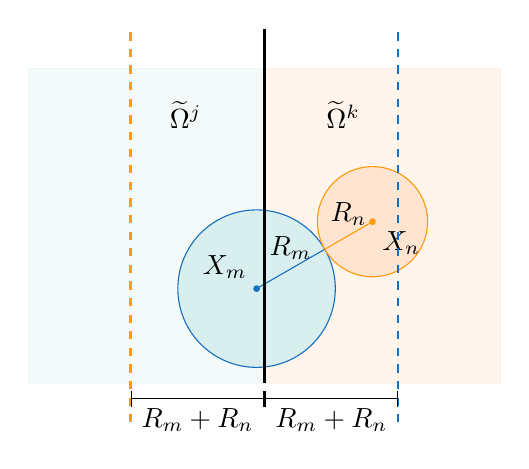
\begin{tikzpicture}

\coordinate (P1) at (-.1,1.2);
\coordinate (P2) at ($(P1) + (30:1.7)$);

\filldraw [tuerkis, opacity=.3] (-3,0) rectangle (0,4);
\filldraw [antituerkis, opacity=.4] (0,0) rectangle (3,4);

\draw [RoyalBlue, fill=tuerkis] (P1) circle (1);
\draw [RoyalBlue, fill=RoyalBlue] (P1) node [above left, black] {$\bm{X}_m$} circle (1pt);

\draw [RoyalBlue] (P1) -- node [above, black] {$R_m$} ++(30:1);

\draw [darkantituerkis, fill=antituerkis] (P2) circle (.7);
\draw [darkantituerkis, fill=darkantituerkis] (P2) node [below right, black] {$\bm{X}_n$} circle (1pt);

\draw [darkantituerkis] (P2) -- node [above, black] {$R_n$} ++(210:.7);

\draw (-1,3.4) node {$\widetilde{\Omega}^j$};
\draw ( 1,3.4) node {$\widetilde{\Omega}^k$};

\draw [-, thick] (0,0) -- (0,4.5);
\draw [-, thick, dashed, RoyalBlue] (1.7,-.5) -- (1.7,4.5);
\draw [-, thick, dashed, darkantituerkis] (-1.7,-.5) -- (-1.7,4.5);

\draw [|-|] (0,-.2) -- node [below] {$R_m+R_n$} ++(1.7,0);
\draw [|-|] (0,-.2) -- node [below] {$R_m+R_n$} ++(-1.7,0);

\end{tikzpicture}
\end{document}
